\documentclass[a4paper, fontsize=14pt]{extreport}

\usepackage{hyperref} %Метаданные для pdf-файла 
\hypersetup{
pdftitle={Решение задач по курсу радиационной физики},
pdfsubject={Радиационная физика},
pdfauthor={Пилипенко Кирилл Сергеевич},
pdfkeywords={Ионизирующее излучение, Дозиметрия, Радиоактивность, Ремизов, 4 курс Медицинская физика}
}

\usepackage[english,russian]{babel}

\usepackage{scrextend}                    % Вжух!
\usepackage{fontspec}                     % и твой шрифт
\setmainfont[Scale=.976]{Times New Roman} % такой, как надо!
\usepackage{setspace}
\linespread{1.4}
\usepackage{indentfirst} %первый абзац
\setlength{\parindent}{1cm} %его настройка

\usepackage{tabularx}
\usepackage{xspace}
\usepackage{amssymb} %нестандартные символы
\usepackage{mhchem} % the canonical chemistry package
% \usepackage{autonum} % нумерация только тех уравнений, на которые идут ссылки

\usepackage{setspace} %интерлиньяж
% одинарный интервал
\singlespacing
\usepackage{icomma}
\usepackage{xcolor}
\usepackage{hyperref}
\definecolor{urlcolor}{HTML}{000000}
\hypersetup{colorlinks=true, urlcolor=urlcolor} % pdfstartview=FitH,  linkcolor=linkcolor, urlcolor=urlcolor,

%  \usepackage{fancyhdr,fancybox}
%   \pagestyle{fancy}
% \fancyhf{}
%  \chead{Overleaf}
% \fancyhead[C]{\thepage hello}
% \renewcommand{\headrulewidth}{0pt} % remove lines as well
% \setlength{\headheight}{15pt}


\usepackage[left=3cm, right=1.5cm, top=2cm, bottom=2cm]{geometry} %bindingoffset=0cm - хер пойми для чего это
\sloppy %Убирает вылазящие формулы с полей страницы
% \tolerance=700 %Делает тоже самое, что и /sloppy, но хреново (нужны большие значения)

%форматирование оформления разделов
\usepackage{titlesec}
% \renewcommand{\thesection}{}
\renewcommand{\thesubsection}{\arabic{subsection}.}
 % \renewcommand{\thesubsubsection}{\arabic{subsubsection}.}
\titleformat{\section}[block]{\Large\bfseries\filcenter}{}{1em}{}
% \titleformat{\subsusbsection}[block]{\Italic\filleft}{}{1em}{}
% \titleformat*{\subsubsection}{\textit}
\usepackage{graphicx}
\graphicspath{{images/}}
\DeclareGraphicsExtensions{.pdf,.png,.jpg}

\title{Решение задач по курсу радиационный физики }
\author{Пилипенко К.С.}
\date{\today}

\begin{document}
\maketitle
\section{Ионизирующее излучение. Основы дозиметрии }
\textit{Граница спектра тормозного рентгеновского излучения}
\begin{equation} \label{LimitOfSpectrum}
  \lambda = \frac{1,23}{U},
\end{equation}
где U~---~напряжение в рентгеновской трубке, кВ; $\lambda_{min}$, нм.

\textit{Поток рентгеновского излучения}
\begin{equation}
  \textup{Ф} = kIU^2Z,
\end{equation}
где I и U~---~сила тока и напряжения в рентгеновской трубке, Z~---~порядковый номер элемента вещества анода, $k = 10^{-9}B^{-1}$.

\textit{Массовый коэффициент ослабления рентгеновского излучения}
\begin{equation}
  \mu_m = k \lambda^3Z^3,
\end{equation}
где k~---~коэффициент пропорциональности, $\lambda$~---~длина волны, Z~---~порядковый номер вещества-поглотителя.

\textit{Линейный коэффициент ослабления рентгеновского сизлучения}
\begin{equation}
  \mu = \mu_m\rho,
\end{equation}
где $\rho$~---~плотность вещества.

\line(1,0){199}

\textbf{7.1 Найдите границу тормозного рентгеновского излучения (частоту и длину волны) для напряжений $U_1 = 2kB$ и $U_2 = 20kB$. Во сколько раз энергия фотонов этих излучений больше энергии фотона, соответствующего λ = 760 нм (красный цвет)?}
% 	\textit{Решение
% Воспользуемся уравнением \ref{LimitOfSpectrum}, которое связывает приложенное к рентгеновской трубке напряжение U, и минимальную длину волны λ:
% \begin{equation}
% \lambda = \frac{1,23}{U},
% \end{equation},
% где λ — в ангстремах, U – вольтах. Это выражение можно переписать в другом виде. Преобразуем размерность (1):
%
%
% Таким образом, для
% ;.
% Частоты для этих длин волн:
%
%  где с — скорость света. Множитель 109 появился в уравнении из-за того, что мы сразу перевели размерность из нанометров в метры.
% Сравним теперь энергии фотонов с длинами волн λ1,2, λ. Известно, что энергия фотона есть
%
% Тут h – постоянная Планка, ν — частота. Тогда,
%
% Подставим числа:
%
%
% Для отношения энергий:
%
% Ответ: длина волн}

\textbf{7.3 При прохождении потока рентгеновского излучения через костную ткань произошло ослабление в два раза. Учитывая, что толщина слоя костной ткани составляла 20 мм, найдите линейный коэффициент ослабления.}
%  	Решение
% Запишем выражение для потока излучения Ф, прошедшего через слой вещества:
%
% тут Ф0 — первоначальный поток, μ — линейный коэффициент ослабления, x – толщина однородного слоя, которое прошло первоначальное излучение.
% Тогда
%
% откуда:
%
% Подставим числа:
%
% Ответ: линейный коэффициент ослабления μ=34.66 м-1 ≈ 0.035 мм-1.

\textbf{7.7 Сравните изменение массового коэффициента ослабления кости и мягких тканей при переходе от мягкого к жесткому рентгеновскому излучению. Принять энергию фотонов для мягкого излучения равной 30 кэВ, а для жесткого 120 кэВ.} \\
% 	Решение
% Массовый коэффициент ослабления рентгеновского излучения вычисляется как
%
% где k — некотрый коэффициент пропорциональности, λ — длина волны, Z — порядковый номер элемента, из которого сделан поглотитель рентгеновского излучения. Видно, что μm при постоянных k и Z может изменяться только за счет изменения длины волны, поэтому
%
% Энергия и длина волны соотносятся по следущему уравнению
%
% Тут h – постоянная Планка, с — скорсть света.  Таким образом, получаем отношения массовых коэффициентов ослабления:
%
% Ответ: массовый коэффициент ослаления уменьшается в 64 раза при увеличении энергии рентгеновского с 30кэВ до 120 кэВ.

\textbf{7.17 Тело поглотило фотоны рентгеновского излучения с энергией 100 эВ, что значительно превышает энергию ионизации атомов данного вещества. Считая основным эффектом взаимодействие рентгеновского излучения с веществом когерентное рассеяние, найдите длину волны вторичного рентгеновского излучения, если вторичные электроны движутся со скоростью $3,7 \times 10^6$ м/с.}

\textit{Решение.\\
%
}

\textbf{7.20 Считая, что поглощение рентгеновского излучения не зависит от того, в каком соединении атом представлен в веществе, определите, во сколько раз массовый коэффициент ослабления кости $Ca(PO_4)_2$ больше массового коэффициента ослабления воды? }

\textit{Решение.\\
%
\begin{equation}
  Z_{Ca(PO_4)_2}^3 = N_{Ca}Z_{Ca}^3+N_{P}Z_{P}^3+N_{O}Z_{O}^3
\end{equation}
\begin{equation}
  \frac{\mu_m^k}{\mu_m^k} = \frac{N_{Ca}Z_{Ca}^3+N_{P}Z_{P}^3+N_{O}Z_{O}^3}{N_{H}Z_{H}^3+N_{O}Z_{O}^3} = \frac{1 \cdot 20^3 + 2 \cdot 31^3 + 8 \cdot 16^3}{2 \cdot 1^3 }
\end{equation}
Ответ: массовый коэффициент ослабления примерно в 36 раз больше, чем для воды
 }

{\textbf{7.21 Для рентгенодиагностики мягких тканей применяют контрастные вещества. Например, желудок и кишечник заполняют кашеобразной массой сульфата бария $BaSO_4$. Сравните массовые коэффициенты ослабления сульфата бария и мягких тканей (воды). }
Решение
\section{Ядро. Радиоактивность}
\textit{Энергия связи ядра}
\begin{equation}
  \Delta E_\textup{св.} = 931,5[Zm_H + (A - Z)m_n - m_a],
\end{equation}
где $m_H$, $m_n$, $m_a$~---~массы соответственно изотопа водорода $^1H$, нейтрона и атома, а. е. м.; Z~---~число протонов в ядре (порядковый номер элемента), A~---~число нуклонов в ядре (массовое число); $\Delta E_\textup{св.}$ выражается в мегаэлектрон-вольтах.

\textit{Основной закон радиоактивного распада}
\begin{equation}
  N = N_0 e^{-\lambda t},
\end{equation}
где $N_0$~---~начальное число радиоактивных ядер, N~---~их число к моменту времени $t$.
\begin{equation} \label{DecayConst}
  \lambda = \frac{ln2}{T_{1/2}}
\end{equation}
~---~постоянная распада, $T_{1/2}$~---~период полураспада.

 \textit{Изменение активности препарата со временем $[A] = 1\: \text{Ки} = 3,7 \cdot 10^{10} c^{-1}$ Бк (Беккерель)}
 \begin{equation}
   A = \frac{dN}{dt} = \lambda N_0 e^{-\lambda t}.
 \end{equation}
\line(1,0){199}

\textbf{7.31 Выразите через постоянную $\lambda$ распада или период полураспада $T_{1/2}$: а) вероятность того, что радиоактивное ядро распадётся за время от 0 до t; вероятность того, что радиоактивное ядро распадётся за время от t до бесконечности; б) среднее время жизни радиоактивного ядра.}

\textit{Решение \\
%
}

\textbf{7.35 Возраст древних деревянных предметов можно приближенно определить по удельной массовой активности изотопа \ce{^{14}_6C}  в них. Сколько лет тому назад было срублено дерево, которое пошло на изготовление предмета, если удельная массовая активность углерода в нем составляет $^3/_4$ от удельной массы активности растущего дерева? Период полураспада изотопа \ce{^{14}_6C} равен Т = 5570 лет.}

\textit{Решение \\
%
}

\textbf{7.46 Препарат фосфора \ce{^{32}_{15}P} содержат нерадиоактивные примеси. Определите процентное соотношение радиоактивного и нерадиоактивного фосфора в 10 мг препарата, если его активность равна 25 мкКи.}

\textit{Решение \\
%
}
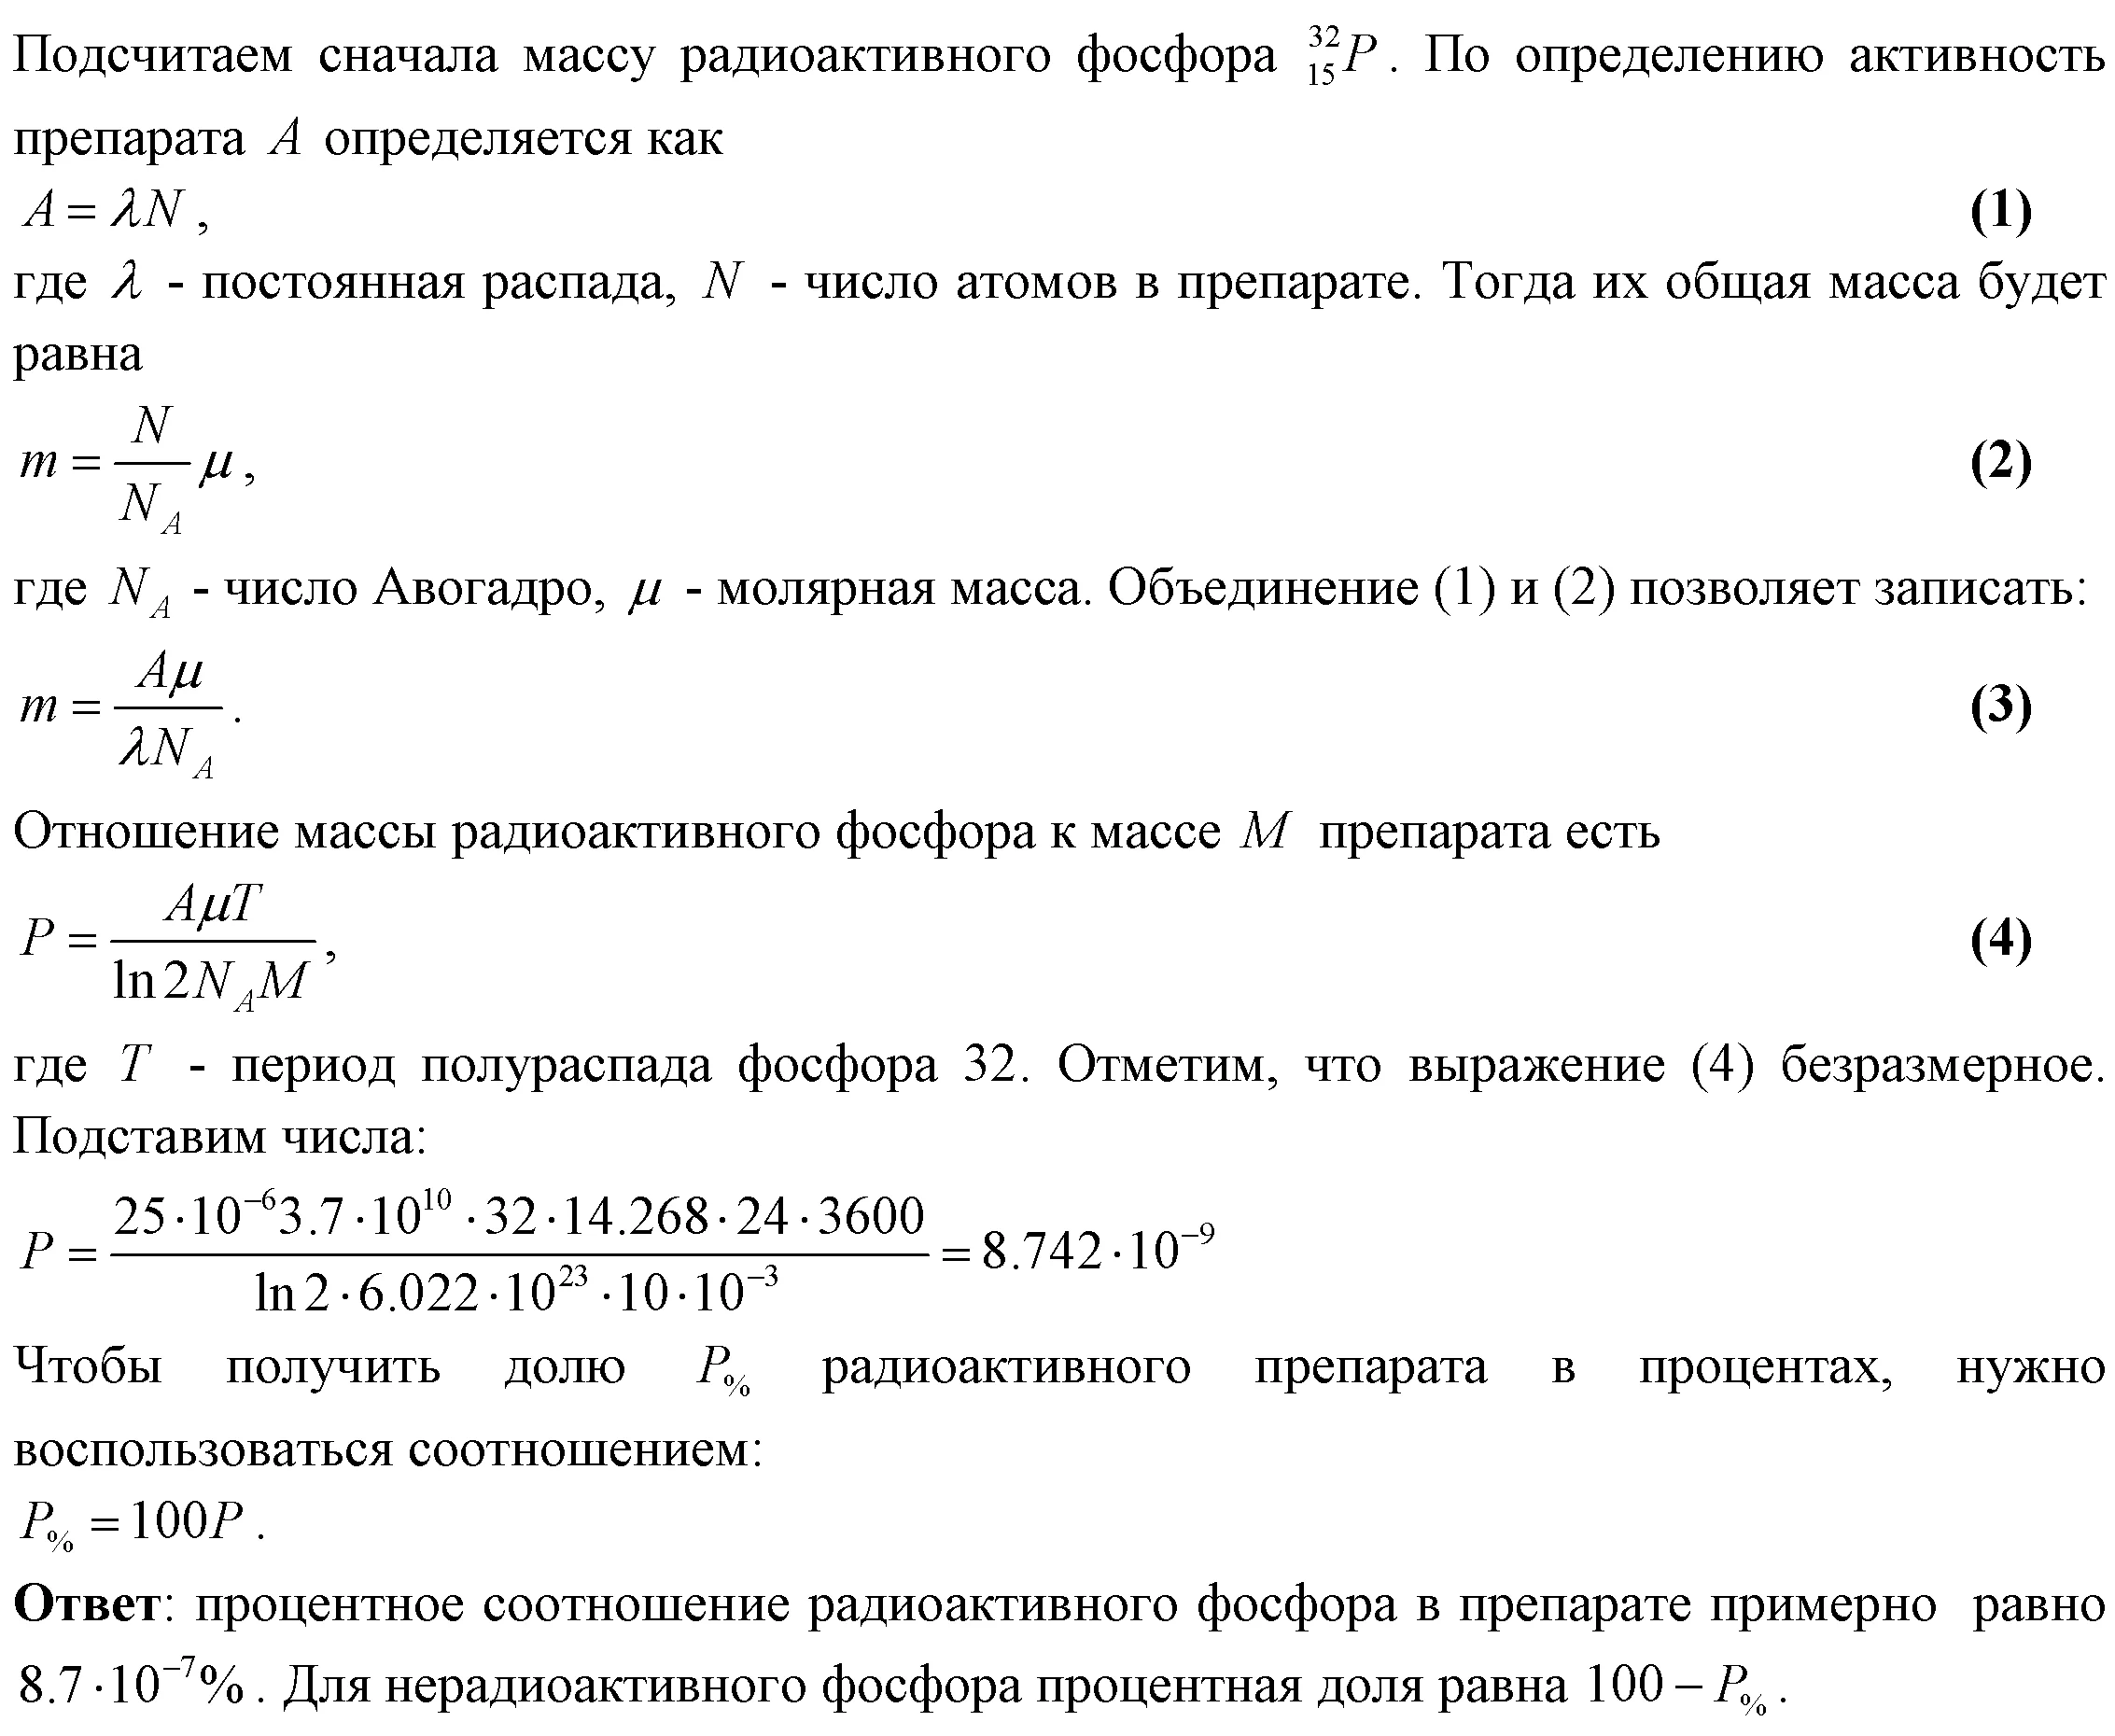
\includegraphics[width=\textwidth]{746}

\textbf{7.48 В 1 мл морской воды содержится $10^{-15}$ г радона \ce{^{222}_{88}Rn} ($T_{1/2} = 3,825 $~суток). Какое количество воды имеет активность, равную 10 мКи?}

\textit{Решение \\
Активность через количество радиоактивных частиц определяется как:
\begin{equation}
  A = \lambda N
\end{equation} 
Используя уравнению \ref{DecayConst} и соотношение $N = \frac{m}{\mu}N_A$ получим активность через период полураспада:
\begin{equation}
  A = \frac{N ln2}{T_{1/2}} = \frac{mN_A ln2}{\mu  T_{1/2}}, 
\end{equation} 
где $\mu$~---~молярная масса радона. 
Если $V_1 \sim m_1$ и $V_2 \sim m_2$, то тогда справедливо следующее:
\begin{equation}
  V_2 = V_1\frac{m_2}{m_1},
\end{equation} 
где $m_2$~---~масса радона с активностью 10млКи. Тогда искомый объём $V_2$ будет равен:
\begin{equation}
  V_2 = V_1\frac{A \mu  T_{1/2}}{N_A m_1 ln2 }.
\end{equation}
Переводя активность в систему СИ ($A_0 = 10 \text{мКи} =3,7 \cdot 10^8\text{Бк}$) получим:
\begin{eqnarray}
  V_2 = 1\text{мл}\frac{3,7\cdot 10^8 \text{с}^{-1} \cdot 226 \text{г} \cdot 3,825 \cdot 24 \cdot 3600 \text{с}}{6,02 \cdot 10^{23} \cdot 10^{-15}\text{г} \cdot ln2}  = 662267,4\cdot 10^{2}\text{мл} \approx 66 \text{м}^3
\end{eqnarray}
}


\textbf{7.52 Для исследования щитовидной железы больному ввели 20 мл 10\%-ного раствора глюкозы с радиоактивным йодом. Удельная активность йода в момент введения составляла 0,08 мкКи/мл. Найдите массу йода в растворе. Учесть, что каждая молекула глюкозы связывает один йод.}

\textit{Решение \\
%
Обозначим объём всего раствора V. Тогда объём $V_1$ глюкозы будет равен
\begin{equation}
  V_1 = \frac{P}{100}V,
\end{equation}
где P~---~выраженное в процентах содержание глюкозы в растворе. Полная активность А йода будет тогда определятся как
\begin{equation}
  A = aV_1 = a \frac{P}{100}V,
\end{equation}
где a~---~удельная активность. С другой стороны, активность А есть
\begin{equation}
  A = \lambda N,
\end{equation}
где $\lambda$~---~постоянная распада, N~---~число атомов. Если умножить отношение $N/N_A$, где $N_A$~---~число Авогадро, на молярную массу $\mu$ радиоактивного йода, то можно получить массу $m$ всего йода в растворе, поэтому:
\begin{equation}
 m = \mu N = \mu \frac{A}{\lambda} = \frac{\mu TaPV}{N_A \cdot 100 \cdot ln2}.
\end{equation}
Подставим числа:
\begin{equation}
 m = \frac{130.906\cdot 10^{-3} \cdot 8.021 \cdot 24 \cdot 3600 \cdot 0.08 \cdot 10^{-6} \cdot 3.7 \cdot 10^{10} \cdot 10 \cdot 20}{6.022 \cdot 10^{23} \cdot 100 \cdot ln2} = 1.29 \cdot 10^{-15} \textup{кг}.
\end{equation}
Ответ: масса йода в препарате примерно равна $1.29 \cdot 10^{-15}$кг.
}
% 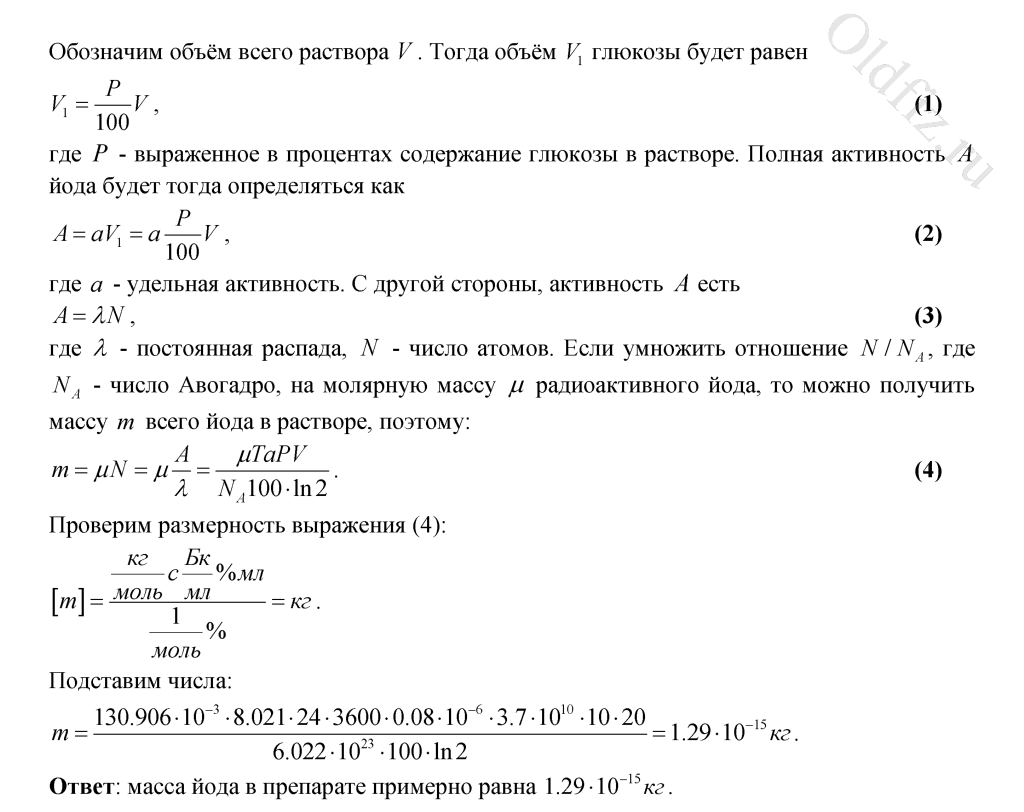
\includegraphics[width=\textwidth]{752}

\section{Основы дозиметрии}
\textit{Удельная активность источника}
\begin{equation}
  A_m = \frac{A}{m},
\end{equation}
где m~---~масса препарата.

\textit{Поглощённая доза}
\begin{equation} \label{absorbDose}
  D = \frac{dE}{dm},
\end{equation}
где $dE$~---~энергия излучения, поглощённая в данном объёме, $m$~---~масса вещества в этом объёме. В СИ: [D] = Дж/кг = Гр(Грей), внесистемные единицы: [D] = 1 рад $=10^{-2}$~Гр.

\textit{Экспозиционная доза}
\begin{equation}
  X = \frac{dQ}{dm},
\end{equation}
$dQ$~---~электрический заряд ионов одного знака, порождённый фотонами в элементарном объёме воздуха, $m$~---~масса воздуха в этом объёме. В СИ: [X] = Кл/кг, внесистемные единицы: [X] = 1 Кл/кг = 3880 Р (рентген).

\textit{Связь поглощённой и экспозиционной доз}
\begin{equation} \label{absorbAndExposition}
  D = fX,
\end{equation}
где f~---~переходный коэффициент (для воды и мягких тканей человека f = 1), если D измеряется в радах, а X~---~в рентгенах.

\textit{Связь эквивалентной и поглощённой доз}
\begin{equation} \label{equivalentDoze}
  H = kD,
\end{equation}
где k~---~коэффициент качества, или относительная биологическая эффективность (ОБЭ). Коэффициент качества для рентгеновского и $\gamma$-излучения равен 1, для $\alpha$-излучения он равен 20.

Предельно допустимая эквивалентная доза для населения составляет 0,05 бэр в год, а для профессионалов она равна 5 бэр в год.

\textit{Связь между активностью радиоактивного препарата (А) и мощностью экспозиционной дозы $X/t$}
\begin{equation} \label{powerExposureDose}
  \frac{X}{t} = k_\gamma \frac{A}{r^2},
\end{equation}
где $k_\gamma$~---~$\gamma$-постоянная, которая характерна для данного радионуклида; r~---~расстояние от источника ионизирующего излучения.

% \textit{Экспозиционная доза измеряется в Кл/кг и рентгенах (Р):}
% \[ 1 \textup{ Р} = 2,58 \cdot 10^{-4}\textup{ Кл/кг}.\]
% Зиверт~---~системная единица измерения эквивалентной дозы. Вводится, чтобы учесть разное биологическое действие разных ионизирующих факторов, поэтому при подсчёте эквивалентной дозы нужно умножить поглощённую дозу на коэффициент К. Например, если рентгеновское излучение с энергией, равной энергии некоторого числа альфа-частиц, пройдёт через живой организм, то вреда от него будет намного меньше, чем от этих же поглощённых альфа-частиц, так как последние при попадании в организм активно вступают в химические реакции, нарушая ход метаболизма. Рентгеновское же излучение в основном ионизирует отдельные атомы, которые после этого возвращаются в исходное состояние, захватив электрон. Таким образом, для рентгеновского излучения К=1, а для альфа-излучения К=20
\noindent \begin{tabularx}
  {\textwidth} { 
  | >{\centering\arraybackslash}X 
  | >{\centering\arraybackslash}X 
  | >{\centering\arraybackslash}X 
  | >{\centering\arraybackslash}X | }
  \cline{2-4}
  \multicolumn{1}{c|}{} & Поглощённая доза $D$ & Экспозиционная доза $X$ & Эквивалентная доза $H$ \\ \hline
  СИ & 1 Дж/кг = 1 Грей (Гр) & Кл/кг & Зиверт(Зв) \\ \hline
  Внесистемые & \begin{tabular}{c} рад \\  1 рад = 10$^{-2}$ Гр  \end{tabular} & \begin{tabular}{c} рентген (Р) \\ 1 Кл/кг = 3880 Р  \end{tabular} & бэр (биологический эквивалент рада) 1~бэр~=~10$^{-2}$~Зв \\ \hline
\end{tabularx}

% \line(1,0){199}

\textbf{7.59 В m = 10 г ткани поглощается $10^9$ $\alpha$-частиц с энергией около Е = 5 МэВ. Найдите поглощенную и эквивалентную дозы. Коэффициент качества $k$ для $\alpha$-частиц равен 20.}

\textit{Решение \\
Полная энергия $Q$ поглощённых $N$ $\alpha$-частиц будет равна
\begin{equation}
  Q = NE.
\end{equation}
Тогда поглощённая доза может быть вычислена как:
\begin{equation}
  D = \frac{NE}{m}.
\end{equation}
Для эквивалентной дозы H по определению \ref{equivalentDoze} можно написать
\begin{equation}
  H = kD = k \frac{NE}{m}.
\end{equation}
Отметим, что коэффициент качества k зависит от и энергии ионизирующих частиц (электронов, $\alpha$-частиц, тяжёлых ионов) или излучений (электромагнитное излучение с малой длиной волны), но и от состава облучаемого образца. Подставим числа из условия задачи:
\begin{equation}
  D = \frac{10^9 \cdot 5 \cdot 10^6 \cdot 1,6 \cdot 10^{-19}}{10 \cdot 10^{-3}} = 8 \cdot 10^{-2} \frac{\textup{Дж}}{\textup{кг}} =8 \cdot 10^{-2} \textup{Гр} = 8 \textup{рад},
\end{equation}
\begin{equation}
  H = 8 \cdot 10^{-2} \cdot 20 = 1,6 \textup{Зиверт} = 160 \textup{бэр}.
\end{equation}
Ответ: поглощённая доза $D = 8 \cdot 10^{-2} \textup{Гр} = 8 \textup{рад}$, эквивалентная доза $H = 1,6 \textup{Зв} = 160 \textup{бэр}$.
}
% 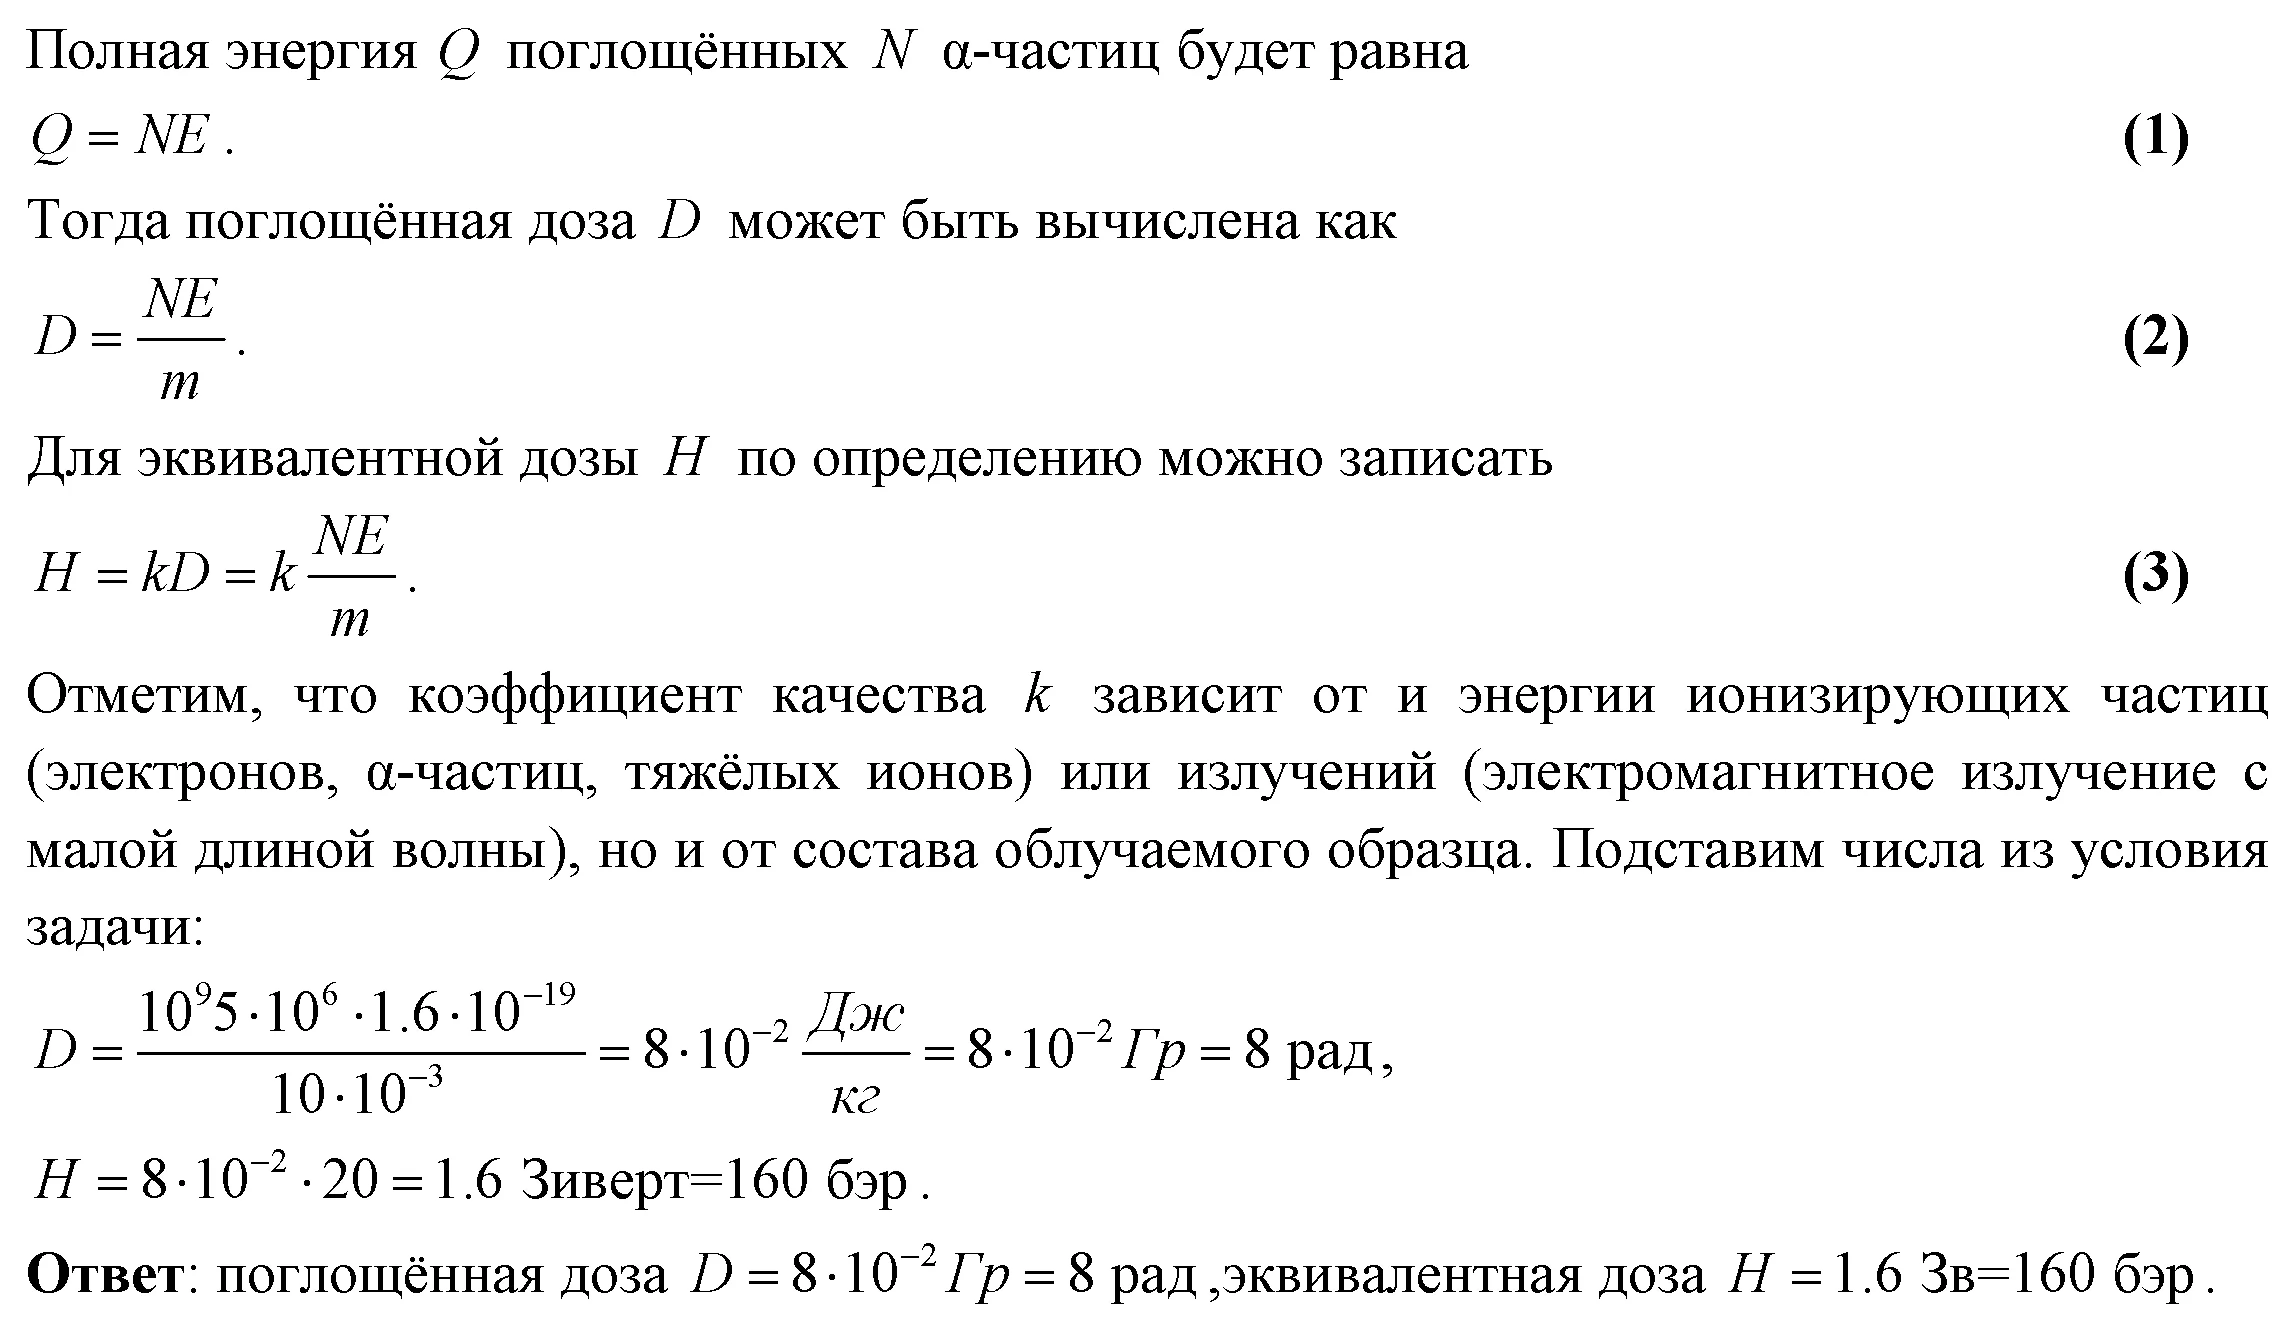
\includegraphics[width=\textwidth]{759}

\textbf{7.60 Мощность экспозиционной дозы  γ-излучения на расстоянии $r_1$~=~1~м от точечного источника составляет $P_1 = 2,15 \times 10^{-7}$~Кл/(кг$\cdot$с). Определите минимальное расстояние от источника ($r_{min}$), на котором можно ежедневно работать по 6 ч без защиты. Предельно допустимой эквивалентной дозой при профессиональном облучении считать $H_{min} = 5 \times 10^{-2}$~Дж/кг в течение года. Поглощение γ-излучения воздухом не учитывать.}

\textit{Решение \\
%
Запишем уравнение \ref{powerExposureDose} для мощности экспозиционной дозы на расстоянии $r_1$ = 1~м
\begin{equation} \label{760Power1}
  P_1 = k_\gamma \frac{A}{r_1^2},
\end{equation}
Для $r_{min}$ соответственно мощность будет равна
\begin{equation} \label{760Power2}
  \frac{X_{min}}{t} = k_\gamma \frac{A}{r_{min}^2},
\end{equation}
Используя уравнения \ref{absorbAndExposition} и  \ref{equivalentDoze} можно получить связь между эквивалентной и экспозиционной дозой в системе СИ:
\begin{equation} \label{760HandX}
  H = \frac{kfX}{38,8}.
\end{equation}
Поделим \ref{760Power1} на \ref{760Power2} с учётом \ref{760HandX}:
\begin{equation}
  \frac{k \cdot f \cdot P_1\cdot t}{H_{min}} = \frac{r_{min}^2}{r_1^2},
\end{equation}
где t~---~время облучения за год, выраженное в секундах. Так как для мягких тканей f = 1, а для $\gamma$-излучения k = 1 то имеем:
\begin{equation}
  r_{min} = r_1 \sqrt{\frac{38,8 \cdot P_1 \cdot t}{H_{min}}}
\end{equation}
}

\textbf{7.61 Средняя мощность экспозиционной дозы облучения в рентгеновском кабинете равна $6,45 \times 10^{-12}$ Кл/(кг·с). Врач находится в течение дня 5 ч в этом кабинете. Какова его доза облучения за шесть рабочих дней?}

\textit{Решение \\
%
Согласно уравнению \ref{powerExposureDose} экспозиционную дозу можно определить как:
\begin{equation}
  X = P\cdot t \cdot n,
\end{equation}
где P~---~мощность экспозиционной дозы, n~---~количество дней, t~---~время облучения в течении дня
Экспозиционная доза X в рентгенах связана с поглощённой дозой D в радах по уравнению \ref{absorbAndExposition}: 
\begin{equation}
  D = f \cdot X,
\end{equation}  
где $f = 1 \frac{\text{рад}}{\text{Р}}$, если мы примем человека за совокупность только мягких  тканей. Эквивалентная доза H определяется из уравнения \ref{equivalentDoze}:
\begin{equation}
  H = kD = k f P n t.
\end{equation}   
Для рентгеновского излучения справедливо $k = 1 \frac{\text{бэр}}{\text{рад}}$.
Поставляя числа получим: 
\begin{equation}
  H =  1 \frac{\text{бэр}}{\text{рад}} \cdot 1 \frac{\text{рад}}{\text{Р}} \cdot \left ( 6,45 \cdot 10^{-12} \cdot 3880\frac{\text{Р}}{\text{c}} \right ) \cdot 6 \cdot 5 \cdot 3600c = 2,7 \cdot 10^{-3} \text{бэр} =  2,7 \cdot 10^{-5} \text{Зв}.
\end{equation}
Ответ: эквивалентная доза равна $H = 2,7 \cdot 10^{-3} \text{бэр} =  2,7 \cdot 10^{-5} \text{Зв}$}

\textbf{7.62 Смертельная доза для человека массой 70 кг при облучении всего тела рентгеновскими или γ-лучами равна 600 рад. На сколько градусов от нормальной поднимется температура тела человека при таком облучении, если считать его однородным фантомом с удельной теплоёмкостью 3,33 кДж/(кг·К)?}

\textit{Решение \\
%
По формуле \ref{absorbDose} имеем следующее:
\begin{equation}
  D = \frac{E }{m}.
\end{equation}
удельная теплоёмкость определяется как:
\begin{equation}
  C_\text{уд.} = \frac{Q}{m\Delta T} 
\end{equation}
Если считать, что вся энергия излучения расходуется на нагрев организма $E = Q$ то изменение температуры можно получить как:
\begin{equation}
  \Delta T = \frac{D\cdot m}{m \cdot C_\text{уд.}} = \frac{D}{C} = \frac{6\cdot \frac{\text{Дж}}{\text{кг}}}{3330 \cdot \frac{\text{Дж}}{\text{кг} \cdot K}} \approx 1,8 \cdot 10^{-3}\: K.  
\end{equation}
Ответ: на  $1,8 \cdot 10^{-3}$~K 
}

\textbf{7.63 Радиационный фон в некотором городе составляет 30 мкР/ч. Определите поглощенную и экспозиционную дозы, полученные жителями этого города в течении года.}

\textit{Решение \\
Экспозиционная доза за время X за время t равна 
\begin{equation}
  X = P \cdot t, 
\end{equation}
где P~---~мощность дозы, t~---~время. Если данный фон обусловлен рентгеновскими или $\gamma$-излучением, то поглощённая доза равна 
\[ D = f \cdot X ,\]
где $f = 1 $ рад/Р. Подставим числа:
\[ X = 30 \cdot 10^{-6} \frac{\text{Р}}{\text{ч}} \cdot 365 \cdot 24\text{ч} = 0,263 \: \text{Р}.
\]
\[ D = 1\frac{\text{рад}}{\text{Р}} \cdot 0,263 \: \text{Р} = 0,263 \: \text{рад}.
\]
Ответ: поглощённая доза D = 0,263 рад, экспозиционная доза X = 0,263 Р.
}

\textbf{7.64 При исследовании радиочувствительности живых организмов крыс облучали рентгеновскими лучами в течение 4 ч. При этом полученная ими суммарная доза составила 300 бэр. Найдите мощность экспозиционной и поглощенной дозы в этом эксперименте (в системе СИ).}

\textit{Решение \\
%
Поглощённая и экспозиционная дозы связаны между собой уравнением \ref{absorbAndExposition}:
\begin{equation}
  D = \frac{H}{k},
\end{equation}
где k~---~коэффициент пропорциональности k = 1 бэр/рад = 1 бэр/рад = 1 Зв/Гр.
Мощность доз D и X можно выразить как:
\begin{equation}
  P_D = \frac{D}{t}; \;\;\; P_X = \frac{X}{t} 
\end{equation}  
}

\textbf{7.72 Интенсивность γ-излучения уменьшилось в шесть раз при прохождении через слой вещества толщиной 5 см. Найдите линейный коэффициент ослабления вещества.}

\textit{Решение \\
%
}

\textbf{7.73 На каком расстоянии от препарата с радием активностью 100 мКи можно находиться, чтобы эквивалентная доза за шестичасовой рабочий день не превышала допустимую за сутки для профессионалов? Иони­зационная постоянная радия $\gamma = 8,4$~Р$\cdot$м$^{2}$/c$\cdot$Ки}

\textit{Решение \\
Предельно допустимая эквивалентная (H) доза для профессионалов составляет 5 бэр в год.
Расстояние можно выразить из уравнения \ref{powerExposureDose} как 
\begin{equation}
  r = \sqrt{k_\gamma\frac{A \cdot t}{X}}
\end{equation}
}

\textbf{7.75 Мощность экспозиционной дозы на расстоянии 10 см от источника составляет 85 мР/ч. На каком расстоянии от источника можно находиться без защиты, если допустимая мощность дозы равна 0,017 мР/ч?}

\textit{Решение \\
%
Отношение мощностей доз равно:
\begin{equation}
  \frac{P_1}{P_2} = \frac{r^2}{r_1^2}
\end{equation}
Отсюда расстояние выражается как:
\begin{equation}
  r = r_1\sqrt{\frac{P_1}{P_2}} = 10\: \text{cm} \sqrt{\frac{85\text{мР/ч}}{0,017\text{мР/ч}}} = 707,1\:\text{см} \approx 7,07\: \text{м}.
\end{equation}
Ответ: расстояние $r \approx 7,07$~м.
}
% 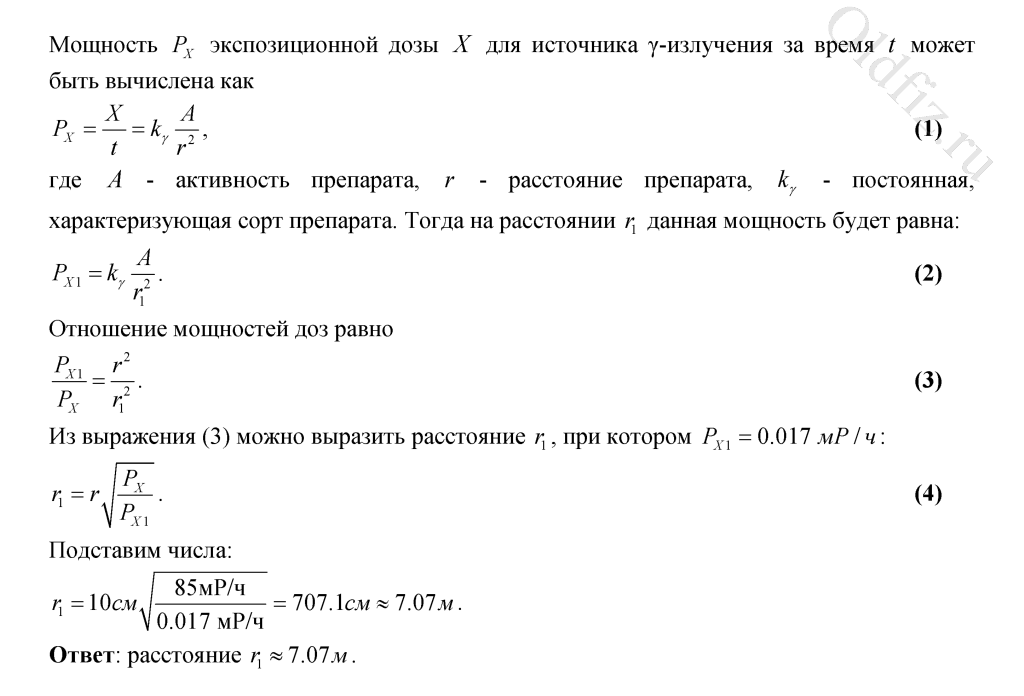
\includegraphics[width=\textwidth]{775}

\end{document}
